\documentclass[12pt]{article}%
\usepackage[T1]{fontenc}%
\usepackage[utf8]{inputenc}%
\usepackage{lmodern}%
\usepackage{textcomp}%
\usepackage{lastpage}%
\usepackage[russian]{babel}%
\usepackage[left=40mm, top=35mm, right=35mm, bottom=35mm, nohead, footskip=10mm]{geometry}%
\usepackage{subcaption}%
\usepackage{graphicx}%
%
%
%
\begin{document}%
\normalsize%
\section{Результаты}%
\label{sec:}%
\subsection{sht38515}%
\label{subsec:sht38515}%


\begin{figure}[h!]%
\begin{subfigure}[b]{0.45\linewidth}%
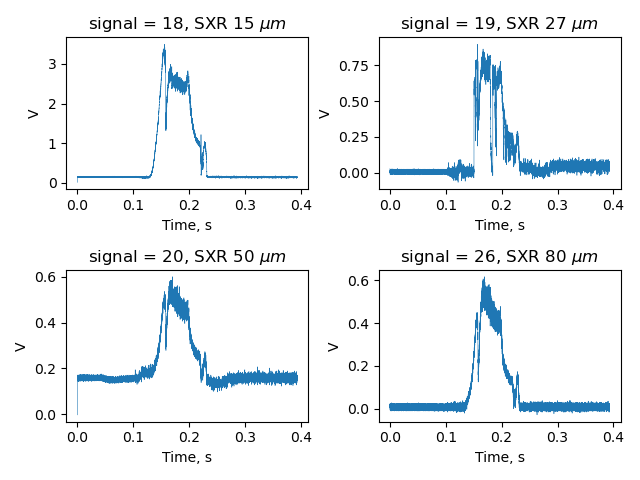
\includegraphics[width=\linewidth]{C:/Users/Limestone/workspace/statistics-cw/MathStat/OUT/raw_sht38515.png}%
\end{subfigure}%
\begin{subfigure}[b]{0.45\linewidth}%
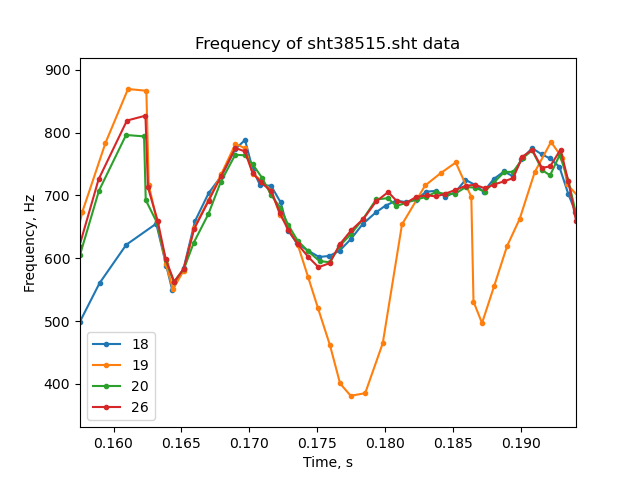
\includegraphics[width=\linewidth]{C:/Users/Limestone/workspace/statistics-cw/MathStat/OUT/sht38515.png}%
\end{subfigure}%
\caption{Сырые данные с показаний датчиков (cлева), Частотный портрет для отобранных сигналов (справа), sht38515}%
\end{figure}

%
\subsection{sht38516}%
\label{subsec:sht38516}%


\begin{figure}[h!]%
\begin{subfigure}[b]{0.45\linewidth}%
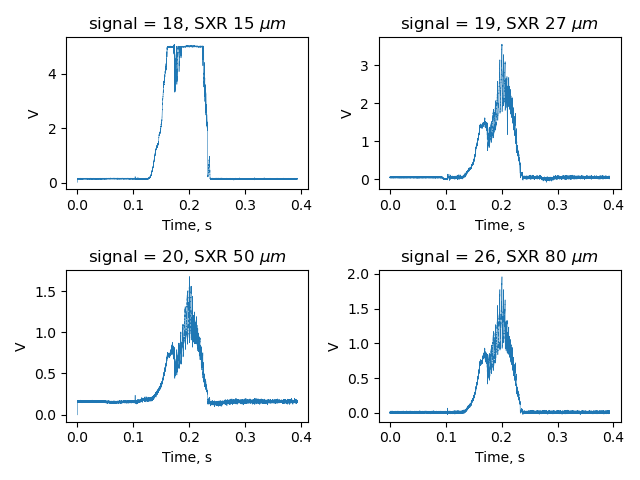
\includegraphics[width=\linewidth]{C:/Users/Limestone/workspace/statistics-cw/MathStat/OUT/raw_sht38516.png}%
\end{subfigure}%
\begin{subfigure}[b]{0.45\linewidth}%
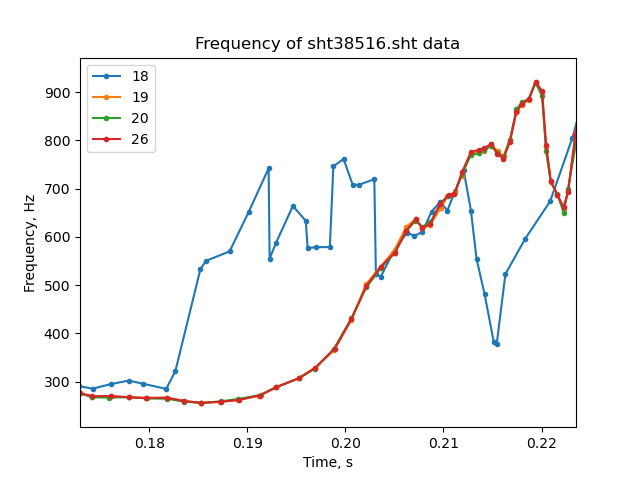
\includegraphics[width=\linewidth]{C:/Users/Limestone/workspace/statistics-cw/MathStat/OUT/sht38516.png}%
\end{subfigure}%
\caption{Сырые данные с показаний датчиков (cлева), Частотный портрет для отобранных сигналов (справа), sht38516}%
\end{figure}

%
\subsection{sht38916}%
\label{subsec:sht38916}%


\begin{figure}[h!]%
\begin{subfigure}[b]{0.45\linewidth}%
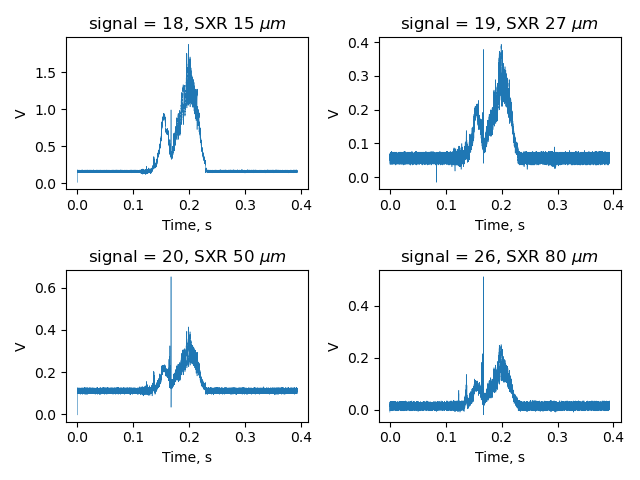
\includegraphics[width=\linewidth]{C:/Users/Limestone/workspace/statistics-cw/MathStat/OUT/raw_sht38916.png}%
\end{subfigure}%
\begin{subfigure}[b]{0.45\linewidth}%
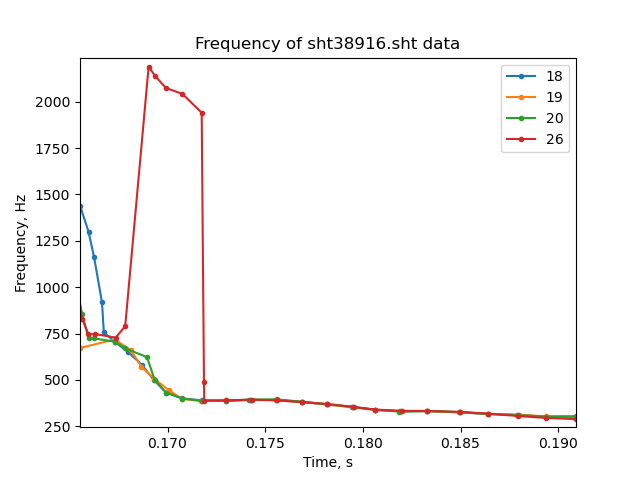
\includegraphics[width=\linewidth]{C:/Users/Limestone/workspace/statistics-cw/MathStat/OUT/sht38916.png}%
\end{subfigure}%
\caption{Сырые данные с показаний датчиков (cлева), Частотный портрет для отобранных сигналов (справа), sht38916}%
\end{figure}

%
\subsection{sht38921}%
\label{subsec:sht38921}%


\begin{figure}[h!]%
\begin{subfigure}[b]{0.45\linewidth}%
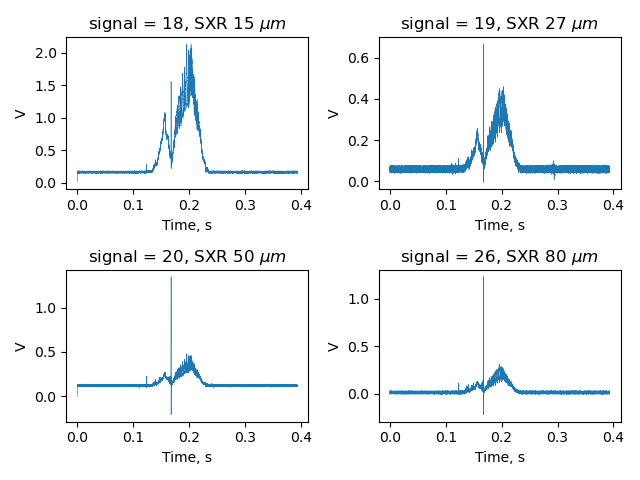
\includegraphics[width=\linewidth]{C:/Users/Limestone/workspace/statistics-cw/MathStat/OUT/raw_sht38921.png}%
\end{subfigure}%
\begin{subfigure}[b]{0.45\linewidth}%
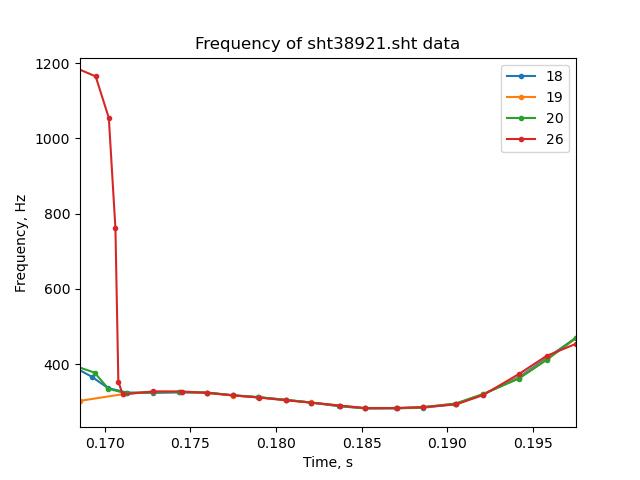
\includegraphics[width=\linewidth]{C:/Users/Limestone/workspace/statistics-cw/MathStat/OUT/sht38921.png}%
\end{subfigure}%
\caption{Сырые данные с показаний датчиков (cлева), Частотный портрет для отобранных сигналов (справа), sht38921}%
\end{figure}

%
\end{document}